\documentclass[aspectratio=169,notes]{beamer}
% \documentclass[aspectratio=169]{beamer}

\mode<presentation>
{
 \usetheme[notitle,noauthor]{Wien} 
%  \usetheme[noauthor]{Wien} 
}

\usepackage[utf8]{inputenc} % Determines encoding of the input. All input files have to use UTF8 encoding.

\usepackage{url}
\usepackage{graphicx}
\usepackage{svg}
\graphicspath{{./}{./graphics/}{./slide-graphics/}}  

\usepackage{appendixnumberbeamer}

% Extended LaTeX functionality is enables by including packages with \usepackage{...}.
\usepackage{amsmath}    % Extended typesetting of mathematical expression.
\usepackage{amssymb}    % Provides a multitude of mathematical symbols.
\usepackage{amsthm}     % theorems
\usepackage{mathtools}  % Further extensions of mathematical typesetting.
\usepackage{complexity} % NP, SAT etc
\usepackage{microtype}  % Small-scale typographic enhancements.
\usepackage[T1]{fontenc} % fonts
% \usepackage{enumitem} % User control over the layout of lists (itemize, enumerate, description).
\usepackage{csquotes}   % Display quotations.
\usepackage{multirow}   % Allows table elements to span several rows.
\usepackage{booktabs}   % Improves the typesettings of tables.
\usepackage{subcaption} % Allows the use of subfigures and enables their referencing.
% \usepackage[usenames,dvipsnames,table]{xcolor} % Allows the definition and use of colors. This package has to be included before tikz.
\usepackage{pgfplots}
\usepackage{standalone} % Allows including standalone content

\usepackage[
% backend=biber,
style=authoryear,
bibstyle=authoryear,
citestyle=authoryear,
% sorting=ynt,
url=false,
isbn=false,
doi=false
]{biblatex}
\addbibresource{bsc_thesis.bib}

\usepackage{frcursive} % 1st slide font

% To avoid a warning from the hyperref package:
\pdfstringdefDisableCommands{%
  \def\translate{}%
}

% To make sure, that the footnote is placed above and outside the
% footline (but it only works for one footnote per frame):
% 
% \addtobeamertemplate{footnote}{}{\vspace{4ex}}

\newcommand\unfootnote[1]{%
  \begingroup
  \renewcommand\thefootnote{}\footnote{#1}%
  \addtocounter{footnote}{-1}%
  \endgroup
}

%%%%%%%%%%%%%%%%%%%%%%%%%%%%%%%%%%%%%%%%%%%%%%%%%%%%%%%%%%%%%%%%%%%%%%%%%%%%% 
%%%%%%%%%%%%%%%%%%%%%%%%%%%%%%%%%%%%%%%%%%%%%%%%%%%%%%%%%%%%%%%%%%%%%%%%%%%%%
\title{Exact and Heuristic Recognition of\\Monotone Lobster Graphs on a Grid}


\subtitle{Bachelor's Thesis}

\author[P. Neubauer]{Peter Neubauer}

\institute[TU Wien]{TU Wien, Vienna, Austria}
   
% \date{\today}
\date{March 14, 2023}

\begin{document}

\begin{frame}
  \titlepage
\end{frame}      

%%%%%%%%%%%%%%%%%%%%%%%%%%%%%%%%%%%%%%%%%%%%%%%%%%%%%%%%%%%%%%%%%%%%%%%%%%%%% %%%%%%%%%%%%%%%%%%%%%%%%%%%%%%%%%%%%%%%%%%%%%%%%%%%%%%%%%%%%%%%%%%%%%%%%%%%%%

\section{Introduction}

%%%%%%%%%%%%%%%%%%%%%%%%%%%%%%%%%%%%%%%%%%%%%%%%%%%%%%%%%%%%%%%%%%%%%%%%%%%%%

\begin{frame}{La Trahison des Images}

\begin{figure}
    \centering
    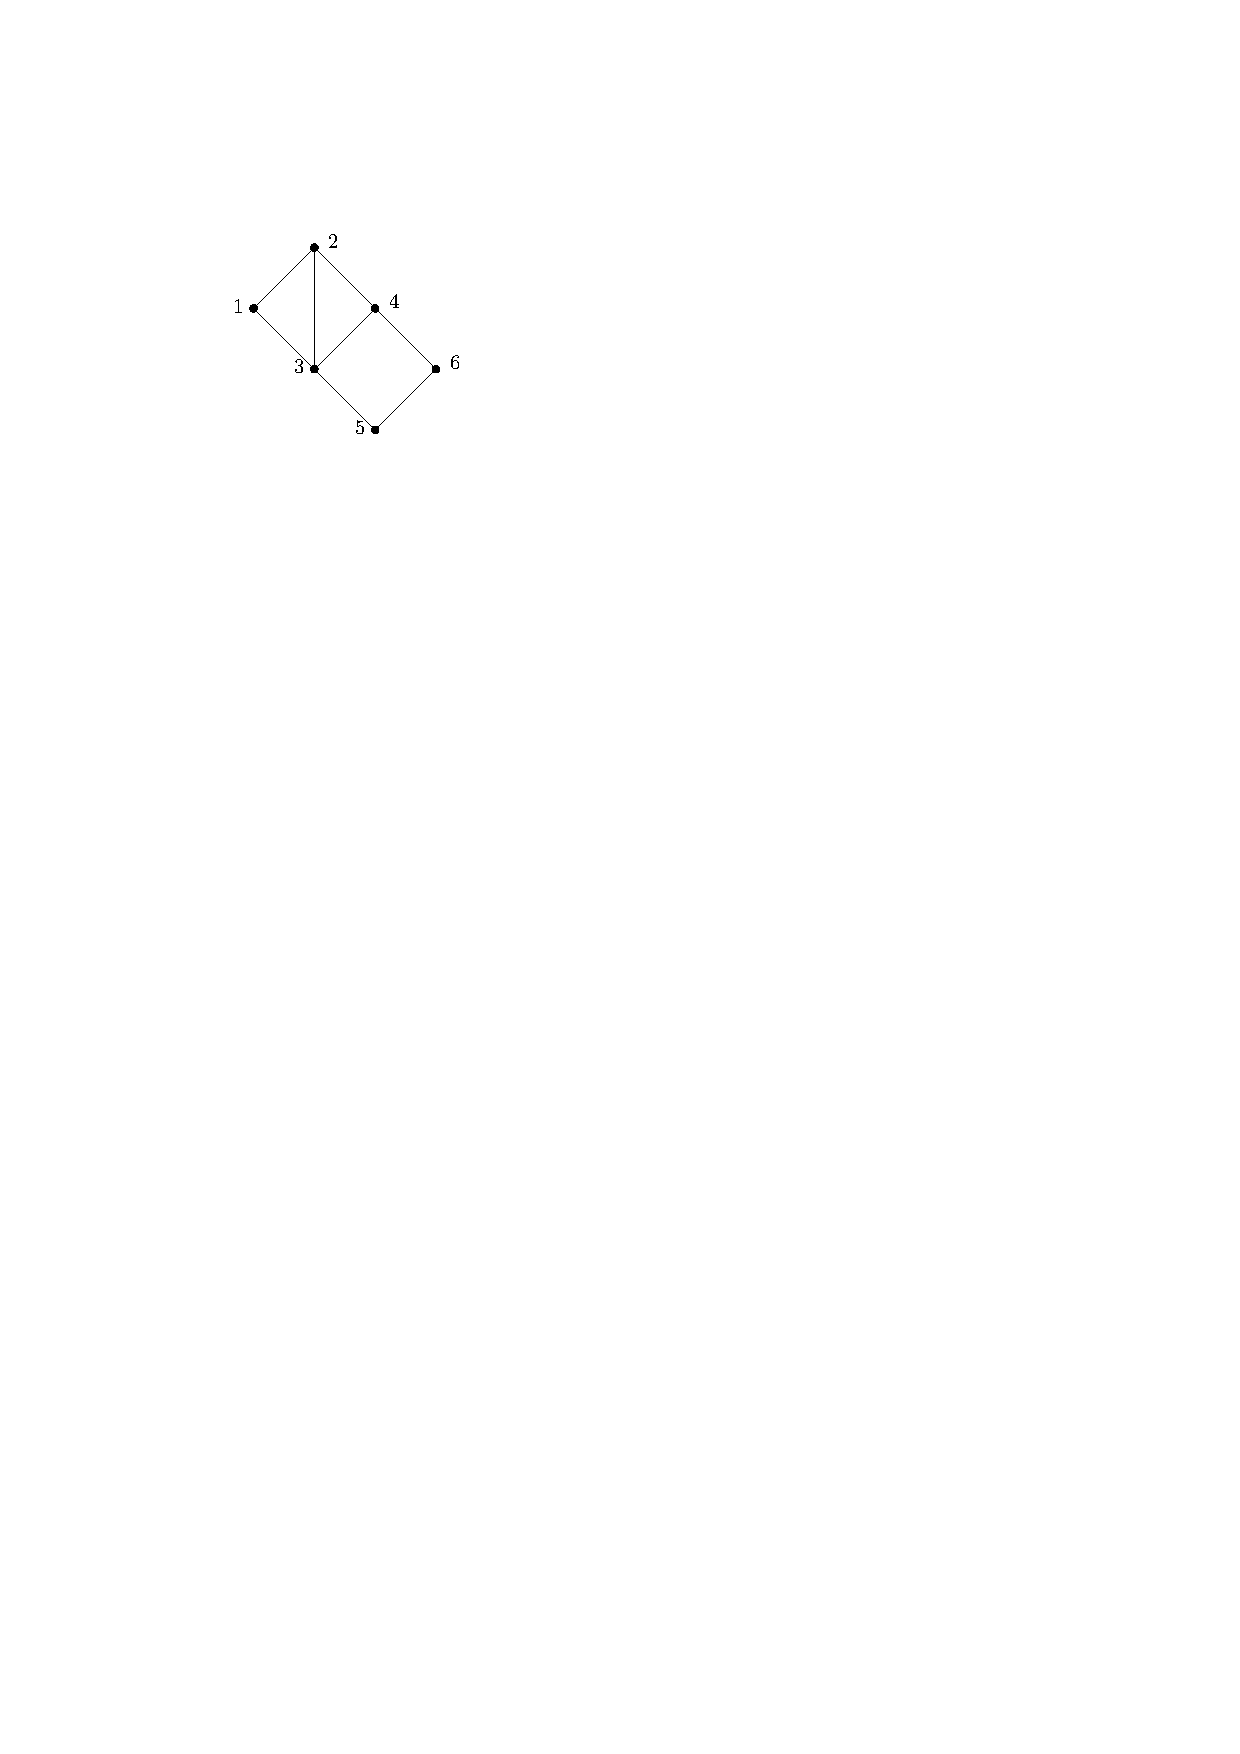
\includegraphics{ch1_introduction_1.pdf}
    \caption*{\fontfamily{frc}\selectfont Ceci n'est pas un graphe}
\end{figure}

\end{frame}

\begin{frame}{Circle Packing Theorem}

\begin{figure}
    \centering
    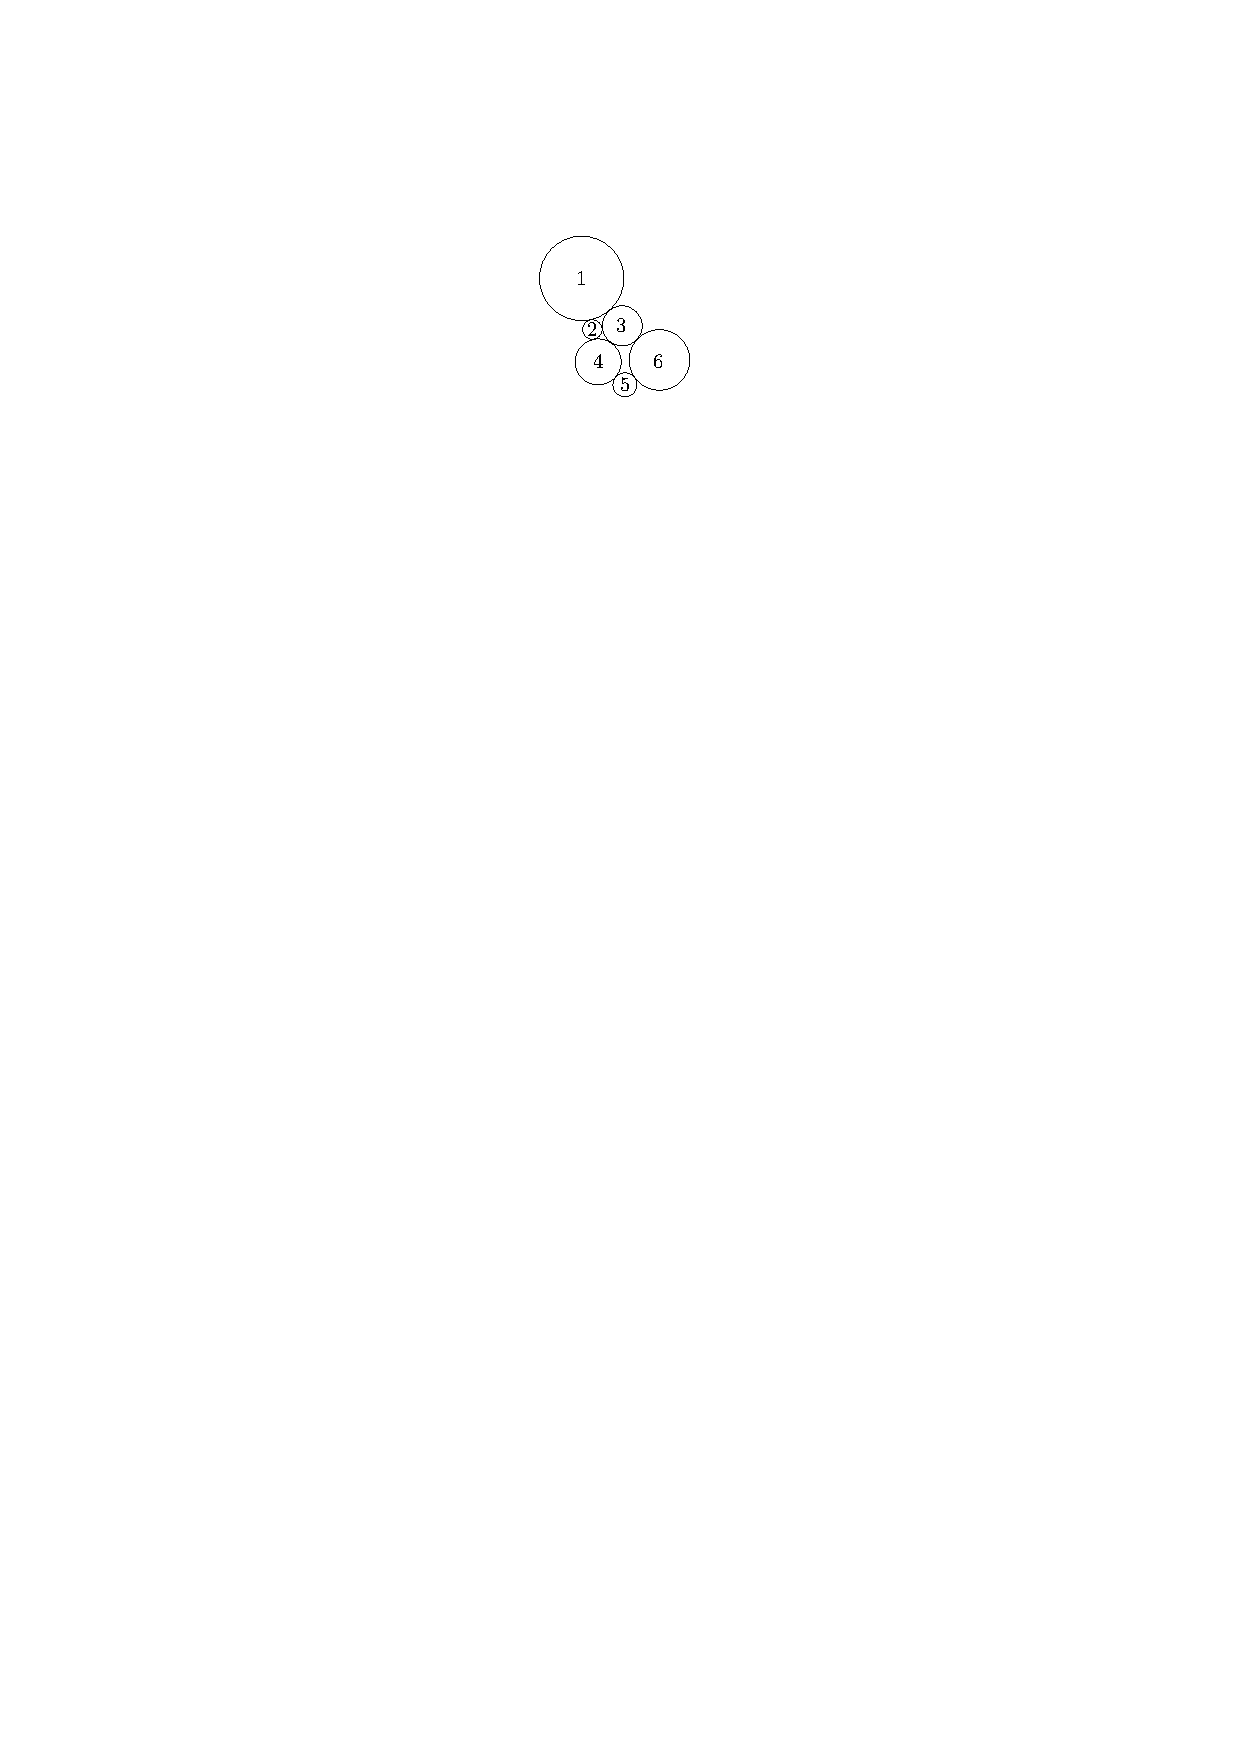
\includegraphics{ch1_introduction_2.pdf}
    \caption*{All planar graphs admit a disk contact representation~(\cite{Koebe1936}).}
\end{figure}

\end{frame}

\begin{frame}{(Weak) Unit Disk Contact}


\begin{columns}
\begin{column}{0.5\textwidth}
    \begin{itemize}
        \item Disks of unit size: $\forall v\,w(v) = 1$
        \item Strict contact: $(u, v) \in E \Longleftrightarrow d(u) \text{ touches } d(v)$
        \item Weak contact: $(u, v) \in E \Longrightarrow d(u) \text{ touches } d(v)$
    \end{itemize}
\end{column}
\begin{column}{0.4\textwidth}
\begin{figure}
    \centering
    
\includegraphics{ch1_introduction_3.pdf}
    \caption*{Recognition problem: does a given graph admit a (weak) unit disk contact representation?}
\end{figure}
\end{column}
\end{columns}


\end{frame}


\section{Related Work}

% \begin{frame}{In Literature...}

% \begin{columns}
% \begin{column}{0.4\textwidth}
%     \begin{figure}
%        \centering
%        \includegraphics[width=0.8\textwidth,page=7,viewport=158 120 346 250,clip]{papers/Kozminski-Rectangular.pdf}
%        \caption*{Any 4-connected, internally triangulated graph admits a contact representation using
% rectangles.}
%     \end{figure}
% \end{column}
% \begin{column}{0.4\textwidth}
% \begin{figure}
%    \centering
%    \includegraphics[width=0.6\textwidth,page=7,viewport=160 410 260 500,clip]{papers/Alam-Tshapes.pdf}
%    \caption*{If the graph is planar triangulated, it admits a contact representation using
% rectilinear polygons with at most 8 vertices.}
% \end{figure}
% \end{column}
% \end{columns}

% \unfootnote{Sources:~\cite{kozminski_rectangular_1985},~\cite{alam_computing_2013}}

% \end{frame}

\begin{frame}{Complexity of Unit Disk Contact Recognition}

\begin{itemize}
\item UDC recognition on general graphs is \NP-hard~(\cite{Breu1998}).
\item Conjecture: UDC recognition on caterpillars can be decided in linear time~(\cite{klemz_recognizing_2022})
\item Weak UDC recognition remains \NP-hard for trees~(\cite{Cleve2020}).
\item Weak UDC recognition on caterpillars is in \P~(\cite{Cleve2020}).
\end{itemize}

\end{frame}

\begin{frame}{Weak Unit Disk Recognition}

\begin{columns}
\begin{column}{0.4\textwidth}
    \begin{figure}
       \centering
       \includegraphics[width=0.8\textwidth,page=2,viewport=260 695 350 745,clip]{papers/Cleve2020-WUDC.pdf}
       \caption*{...can be decided in polynomial time for caterpillars.}
    \end{figure}
\end{column}
\begin{column}{0.4\textwidth}
\begin{figure}
   \centering
   \includegraphics[width=0.7\textwidth,page=7,viewport=90 185 630 705,clip]{papers/Cleve2020-WUDC.pdf}
   \caption*{...remains \NP-hard for trees.}
\end{figure}
\end{column}
\end{columns}

\unfootnote{Source:~\cite{Cleve2020}}

\end{frame}

\begin{frame}{Caterpillar and Lobster}

\begin{figure}
    \centering
    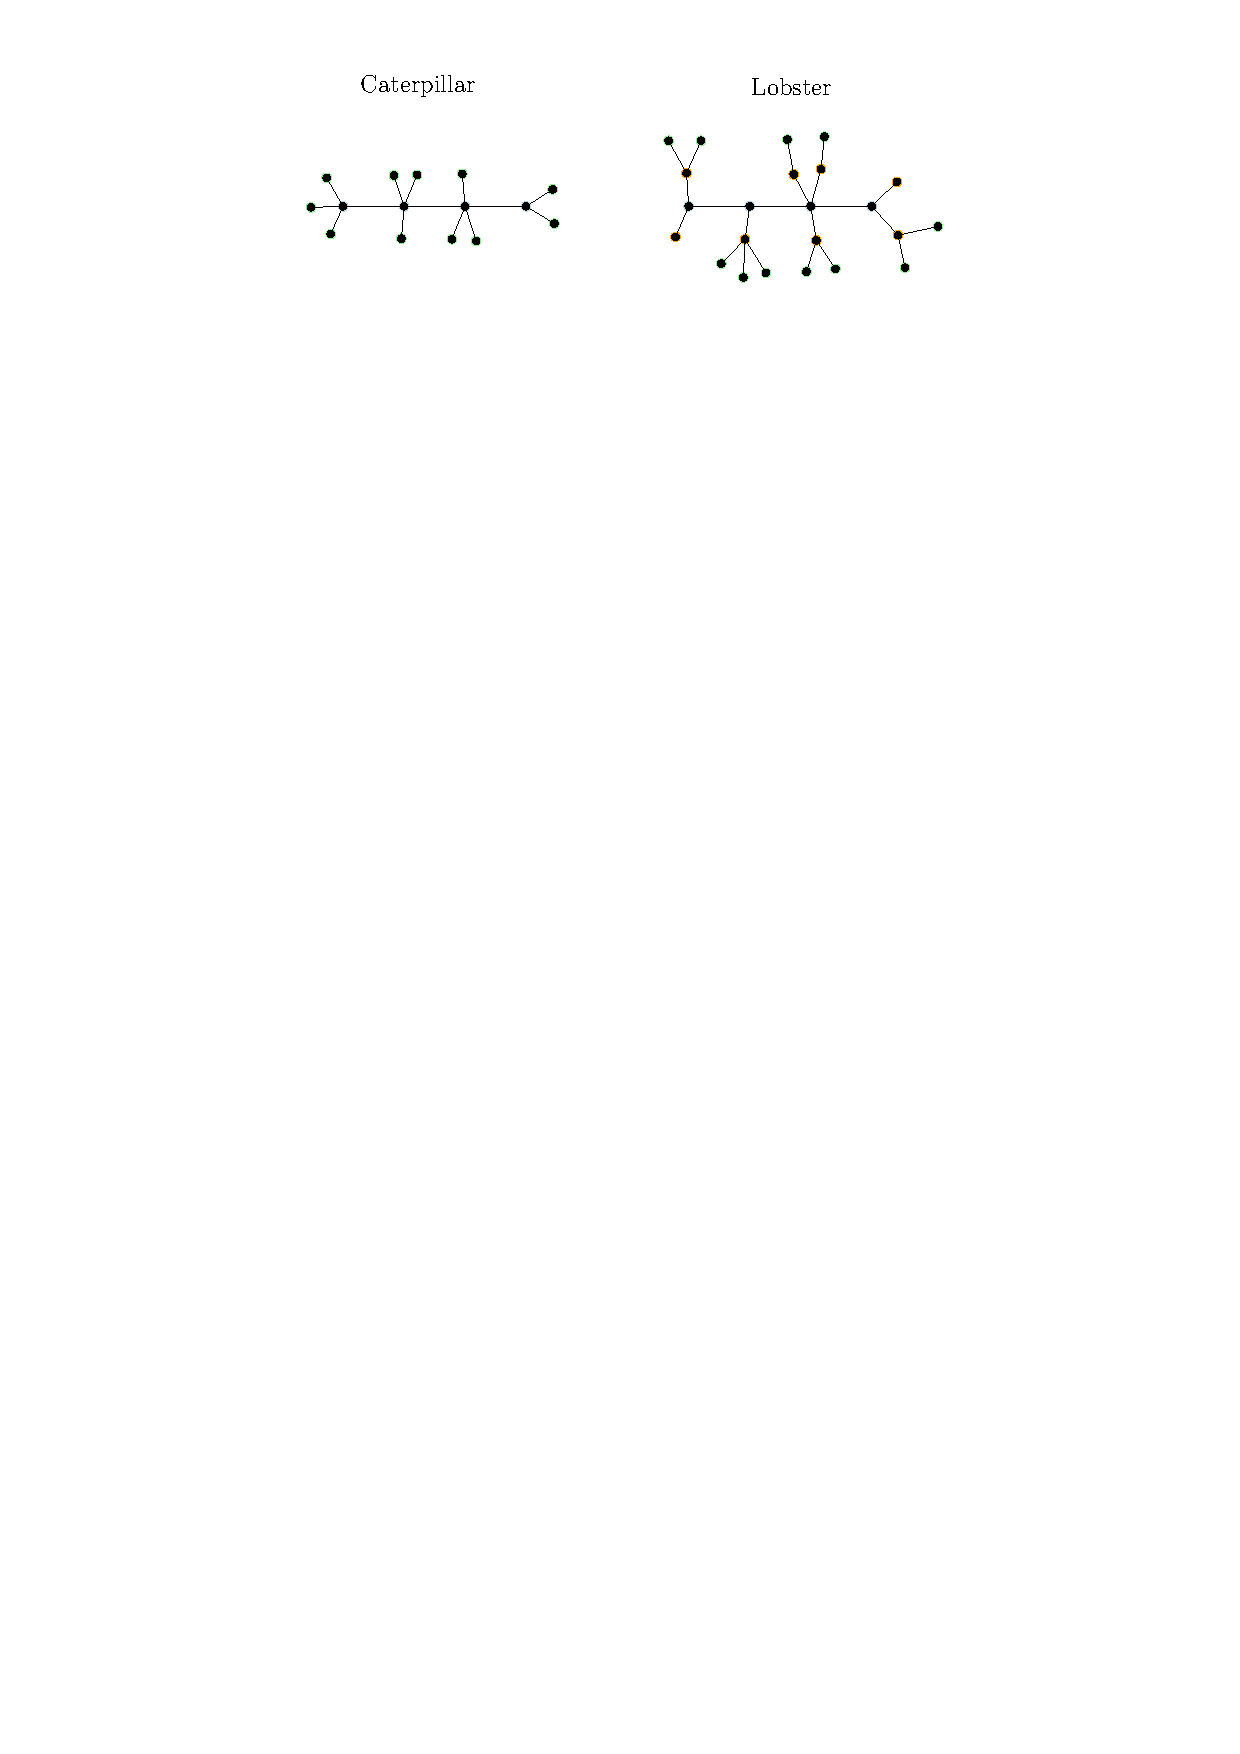
\includegraphics{ch2_caterpillar_lobster.pdf}
   \caption*{A string of \emph{spine vertices} with attached \emph{leaves} (caterpillar) or \emph{branches} with leaves (lobster).}
\end{figure}
    
\end{frame}


\section{Dynamic Program}

\begin{frame}{Monotone Tri-Grid Lobster}

\begin{figure}
    \centering
    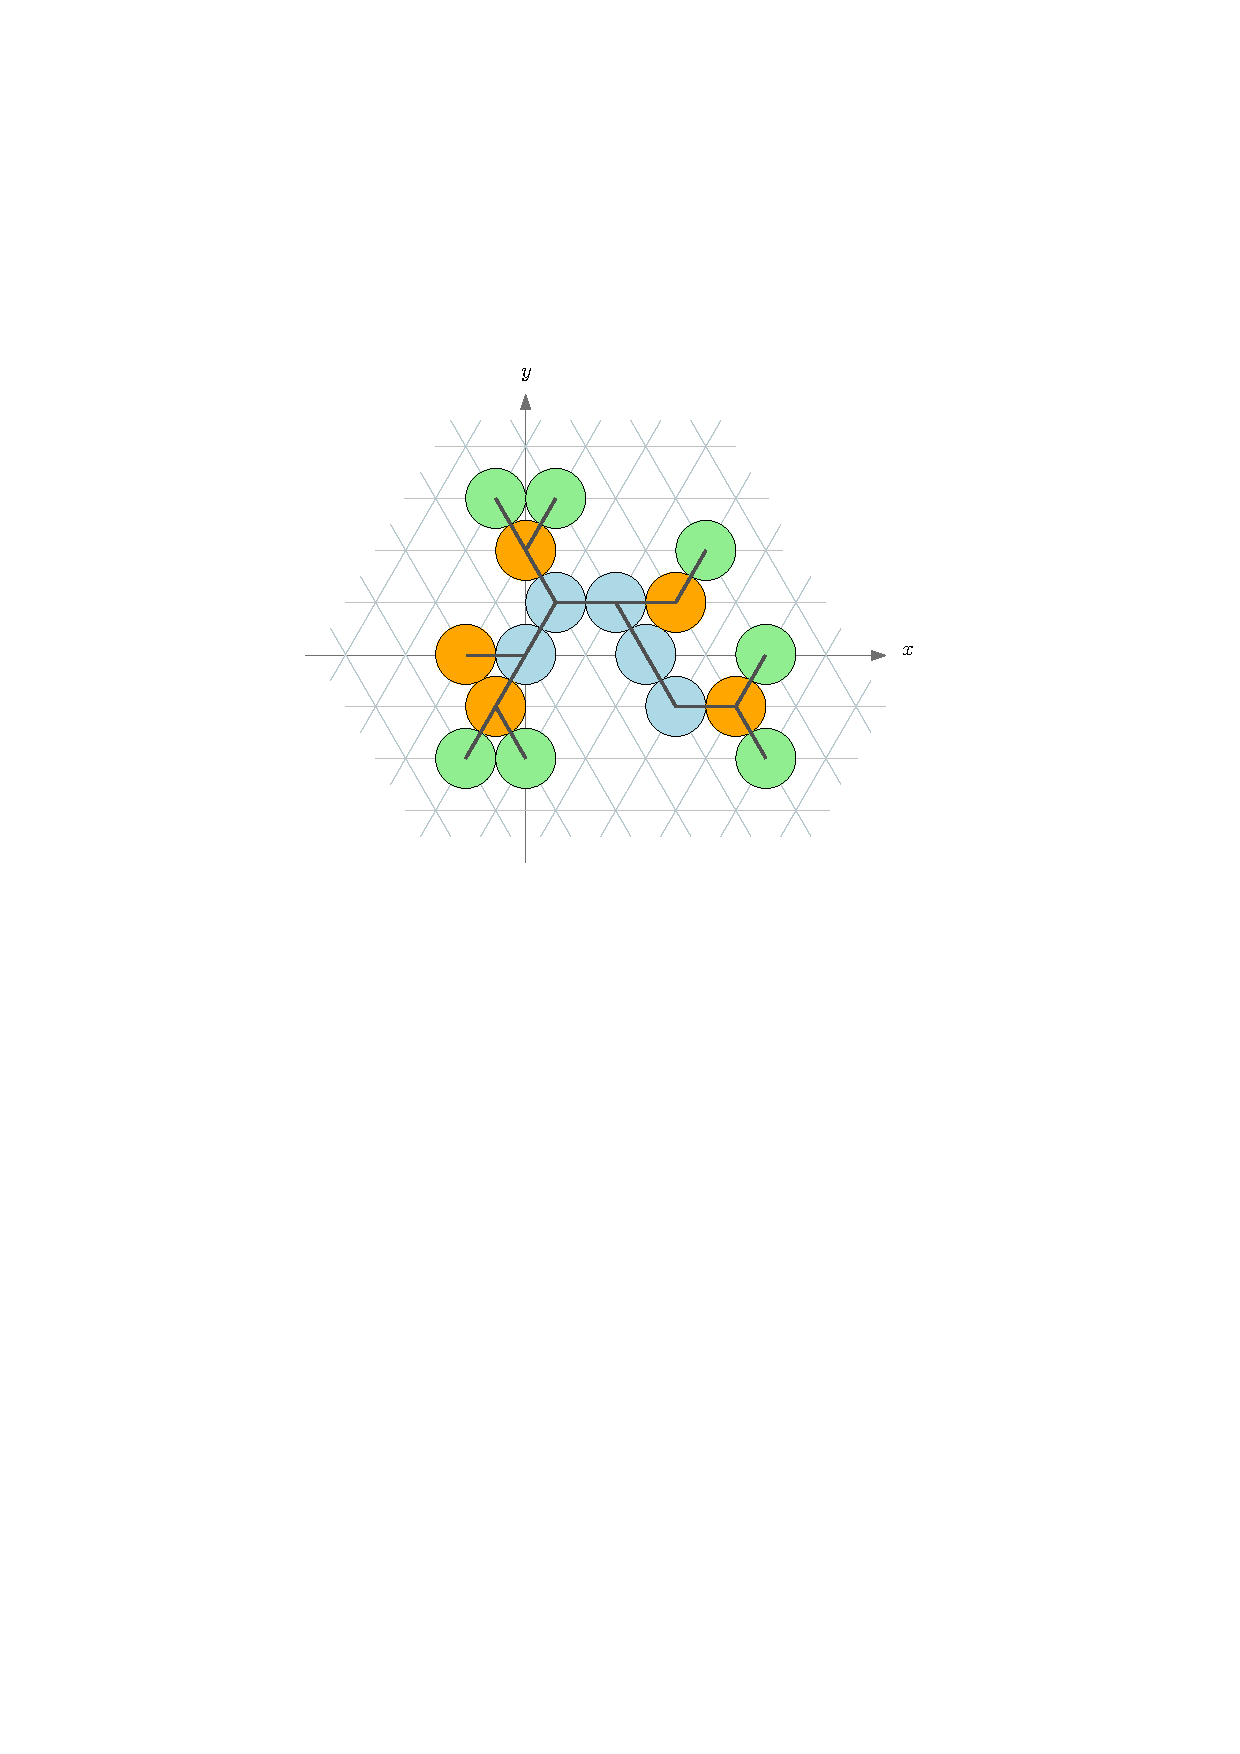
\includegraphics[width=0.5\textwidth]{ch2_tri-grid_x-monotone.pdf}
    \caption*{If a lobster admits an \emph{x-monotone} \emph{tri-grid} UDC representation, \action<+->{we can compute it with a linear-time dynamic programming algorithm~(\cite{Bhore2021}).}}
\end{figure}

\end{frame}

\begin{frame}{Try Everything}

\begin{figure}
    \centering
    \foreach \x in {1,2,3} {%
        \only<\x>{\includegraphics[width=0.5\textwidth,page=\x]{ch4_dpexample_slide.pdf}}
    }
\end{figure}

\end{frame}

\begin{frame}{Example}

\begin{figure}
    \centering
    \only<1>{\includegraphics[width=0.3\textwidth,page=4]{ch4_dpexample_slide.pdf}}
    \only<2>{\includegraphics[width=0.3\textwidth,page=5]{ch4_dpexample_slide.pdf}}
    \only<3>{\includegraphics[width=0.3\textwidth,page=6]{ch4_dpexample_slide.pdf}}
    \only<4>{\includegraphics[width=0.3\textwidth,page=7]{ch4_dpexample_slide.pdf}}
    \only<5>{\includegraphics[width=0.3\textwidth,page=8]{ch4_dpexample_slide.pdf}}
    \only<6>{\includegraphics[width=0.3\textwidth,page=9]{ch4_dpexample_slide.pdf}}
    \only<7>{\includegraphics[width=0.3\textwidth,page=10]{ch4_dpexample_slide.pdf}}
    \only<8>{\includegraphics[width=0.3\textwidth,page=11]{ch4_dpexample_slide.pdf}}
    \only<9>{\includegraphics[width=0.3\textwidth,page=12]{ch4_dpexample_slide.pdf}}
\end{figure}

\end{frame}

\begin{frame}{Dynamic Program}

\begin{columns}
\begin{column}{0.5\textwidth}
    \begin{itemize}
    \item Queue of \emph{signatures}
    \item \emph{Depth} $\delta$: number of disks so far
    \item \emph{Fundament} $F$: blocked spaces nearby
    \item \emph{Spine head} $\gamma_s$: previous spine disk
    \item \emph{Branch head} $\gamma_b$: previous branch disk
    \item Number of possible (constant-size) signatures: $\mathcal O(n)$
    \end{itemize}
\end{column}
\begin{column}{0.4\textwidth}
\begin{figure}
    \centering
    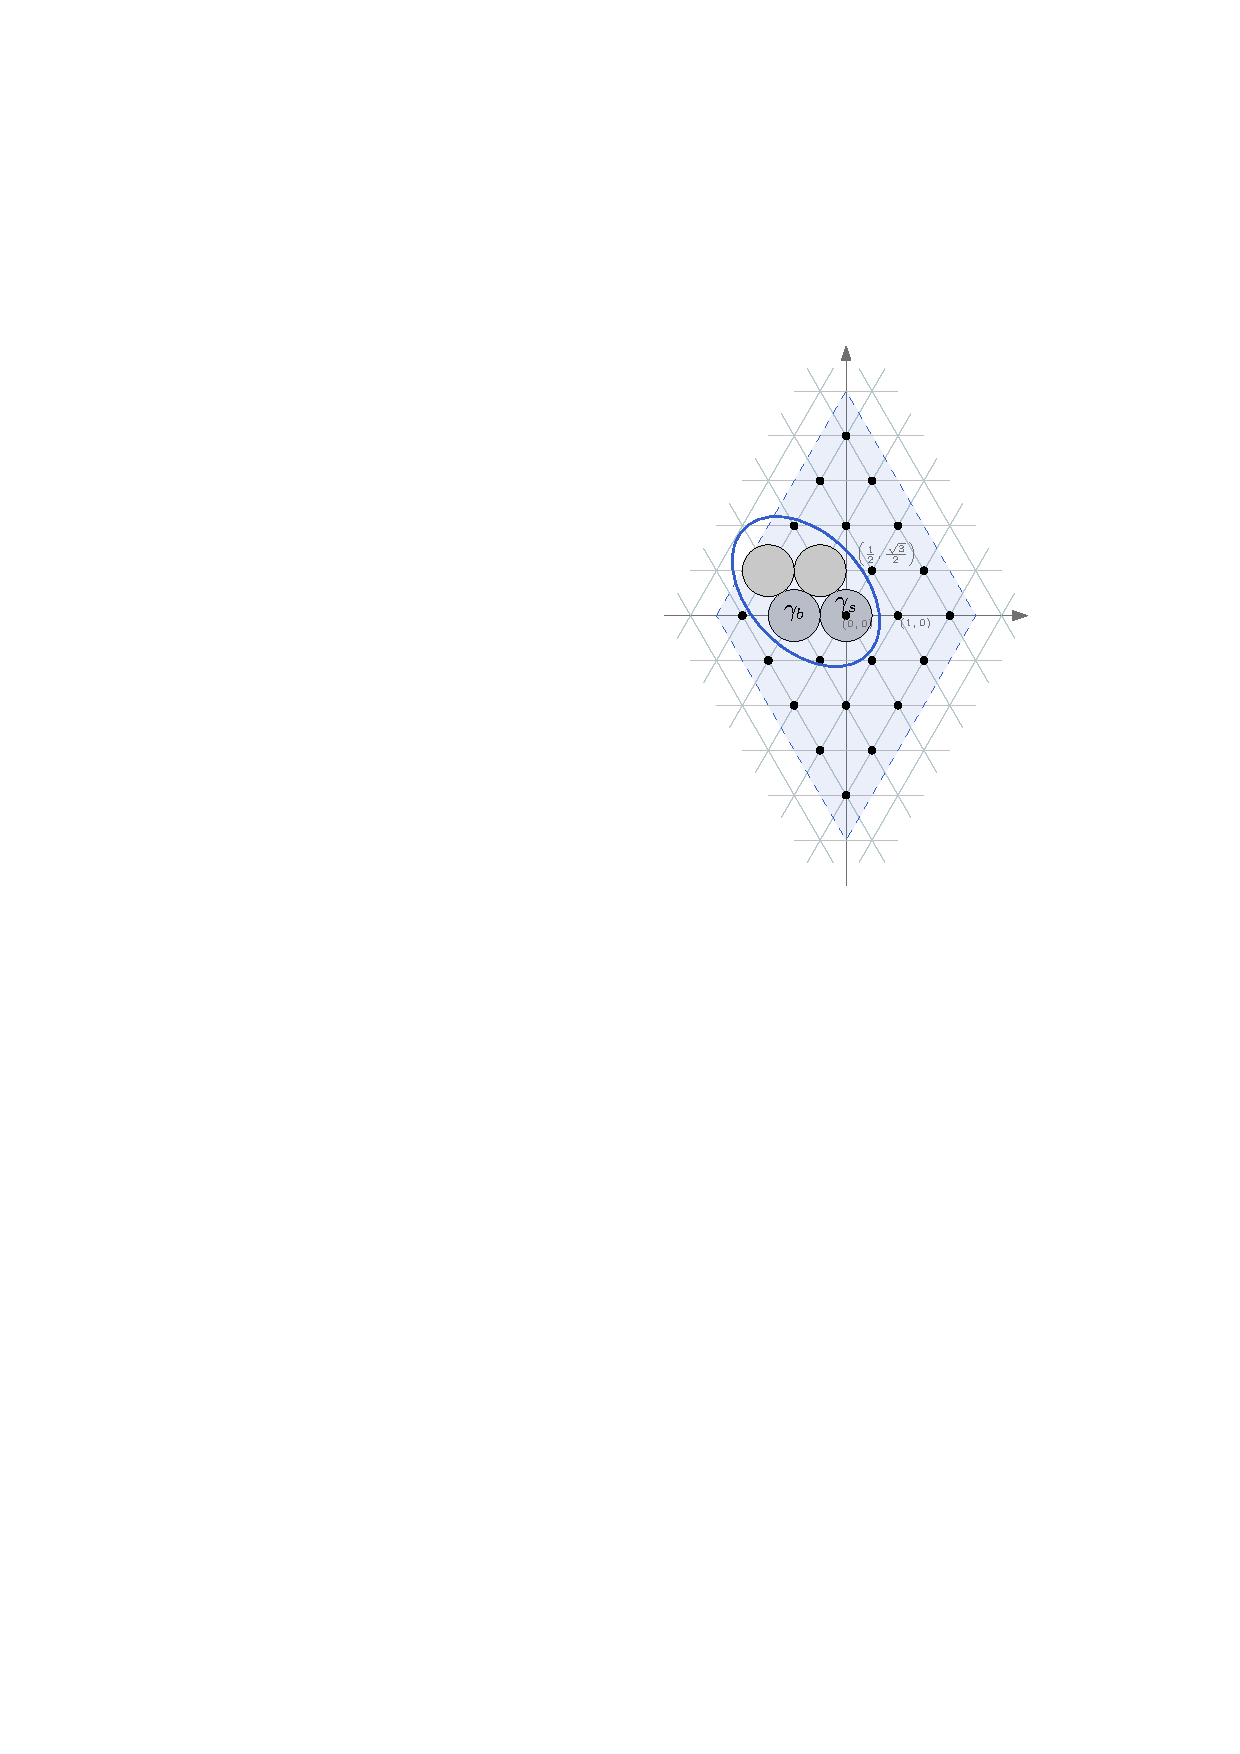
\includegraphics[width=.7\textwidth]{ch4_partialproblem_1.pdf}
\end{figure}
\end{column}
\end{columns}

\end{frame}

\begin{frame}{Improvements}

\begin{columns}
\begin{column}{0.3\textwidth}
\hspace{5em}
    \begin{itemize}
    \item Early Exit
    \item Mirror Instance
    \item Reachability
    \item Domination
    \end{itemize}
\end{column}
\begin{column}{0.5\textwidth}

\begin{table}
\begin{tabular}{@{}cc@{}}
    \scalebox{.7}{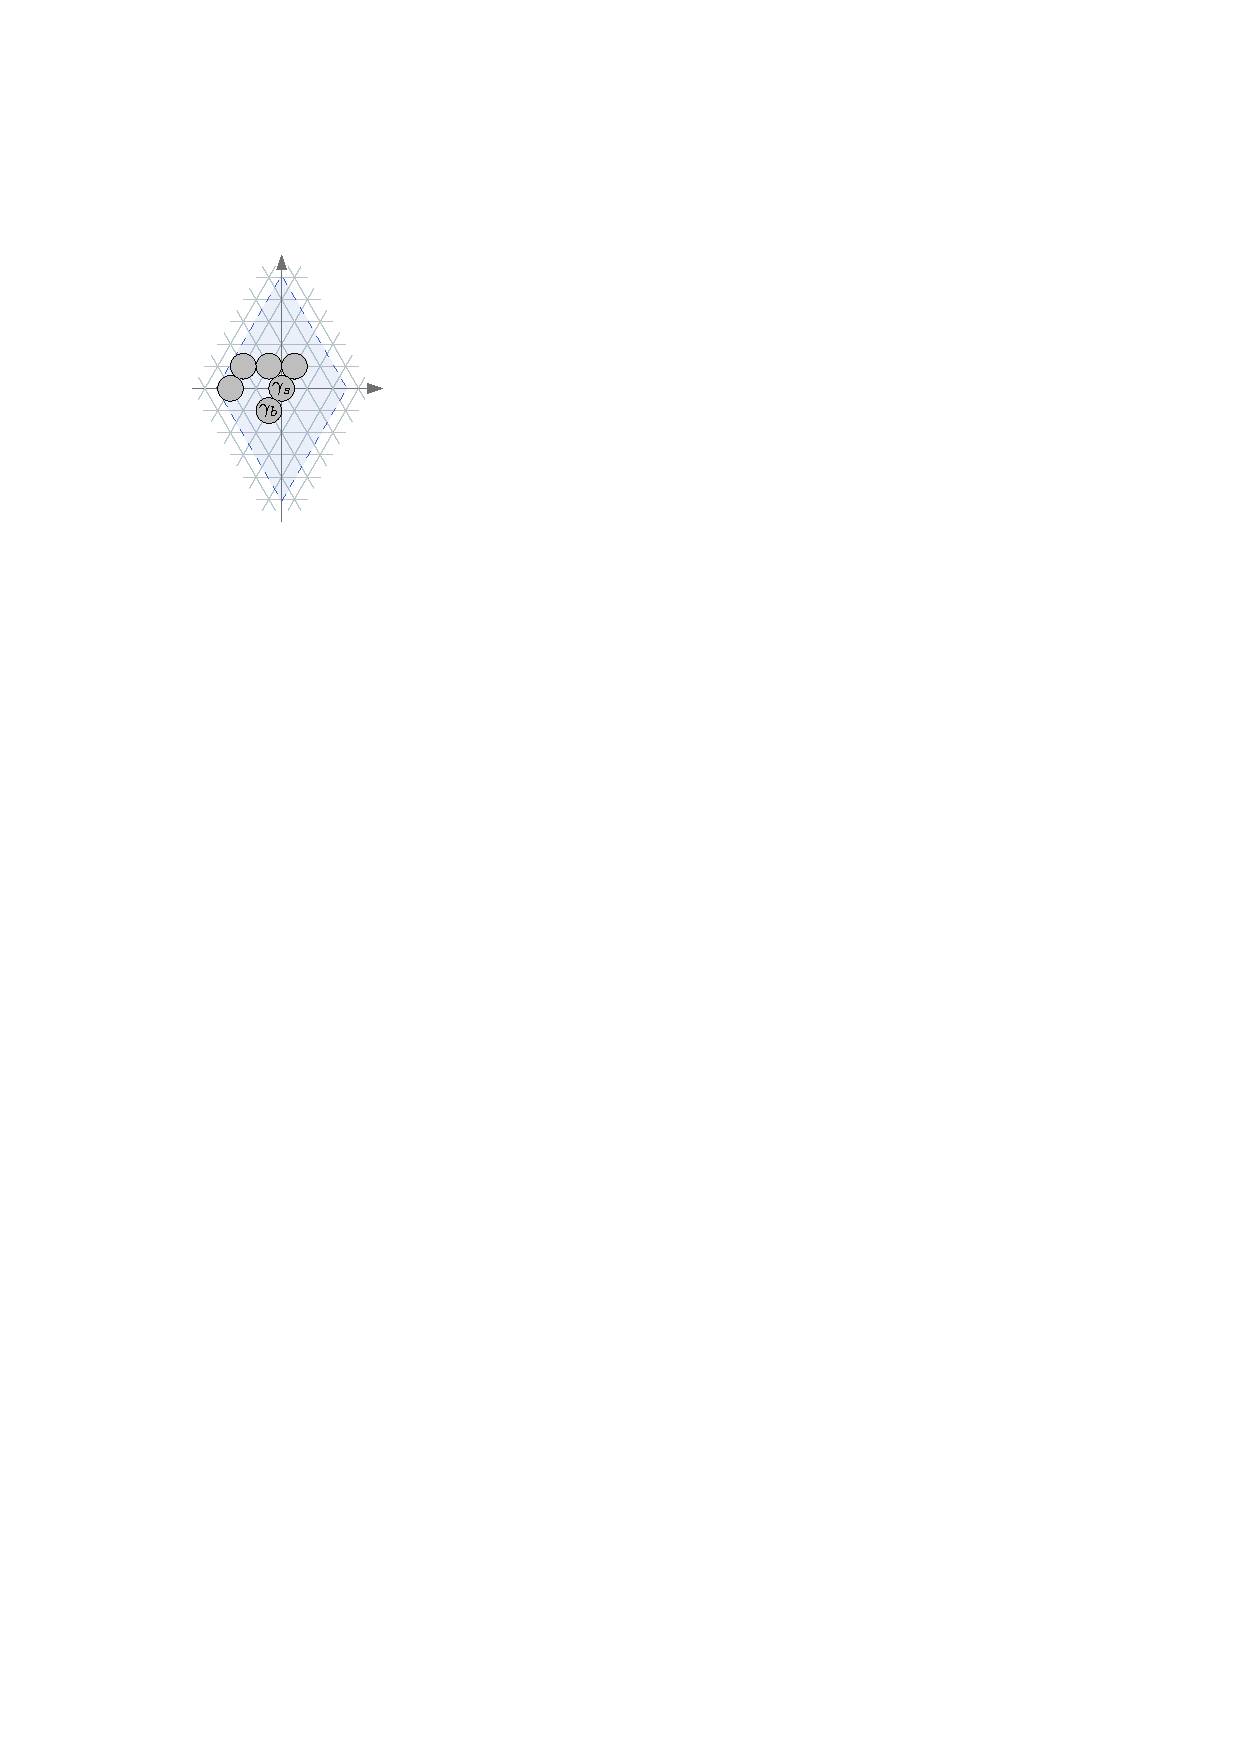
\includegraphics[page=1]{ch4_improvements.pdf}}
    &
    \scalebox{.7}{\includegraphics[page=2]{ch4_improvements.pdf}}
    \\
    \scalebox{.7}{\includegraphics[page=3]{ch4_improvements.pdf}}
    &
    \scalebox{.7}{\includegraphics[page=4]{ch4_improvements.pdf}}
\end{tabular}
\hspace{5em}
\end{table}

\end{column}
\end{columns}

\end{frame}


\section{Heuristic}

\begin{frame}{Heuristic}

\begin{itemize}
\item Greedy
\item Immediately commit to disk placement
\item Spine disks $\rightarrow$ aim for most free space
\item Branch and leaf disks $\rightarrow$ pack tightly \& far back
\item Balance ``load'' above \& below
\end{itemize}

\end{frame}

\begin{frame}{Principal Direction}

\begin{columns}
\begin{column}{0.4\textwidth}
    \begin{itemize}
    \item Decided before each spine disk
    \item Direction of most free space $g$ (weighted)
    \item Branch locations count twice, leaf locations once
    \end{itemize}
\end{column}
\begin{column}{0.4\textwidth}
\begin{figure}
    \centering
    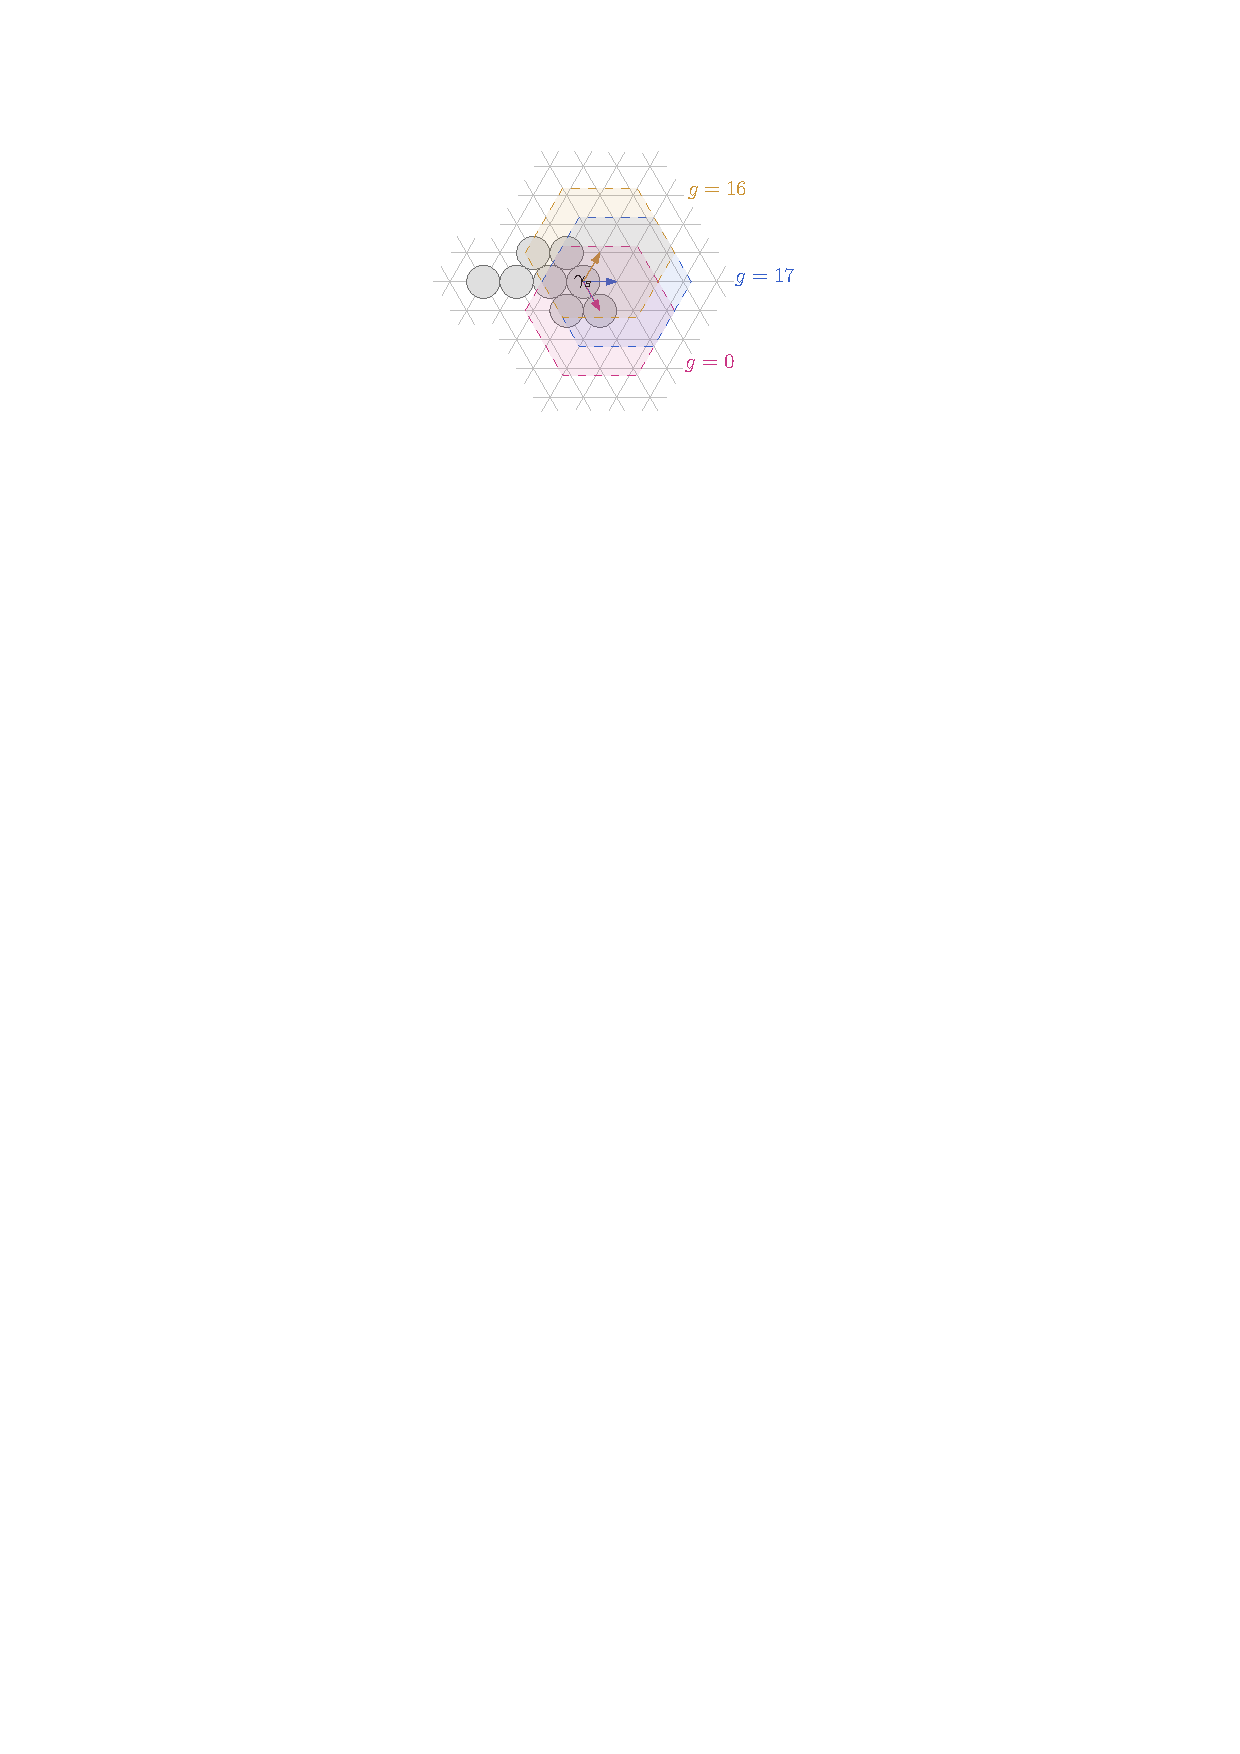
\includegraphics{ch5_principaldirection.pdf}
\end{figure}
\end{column}
\end{columns}

\end{frame}

\begin{frame}{Affinity}

\begin{columns}
\begin{column}{0.45\textwidth}
    \begin{itemize}
    \item Upper placement in $U$ or lower placement in $L$ for each branch and leaf disk
    \item Relative to principal direction $\alpha$
    \item Decision based on most free space
    \item Final disk placement at ``leftmost'' coordinates on the chosen side
    \end{itemize}
\end{column}
\begin{column}{0.4\textwidth}
\begin{figure}
    \centering
    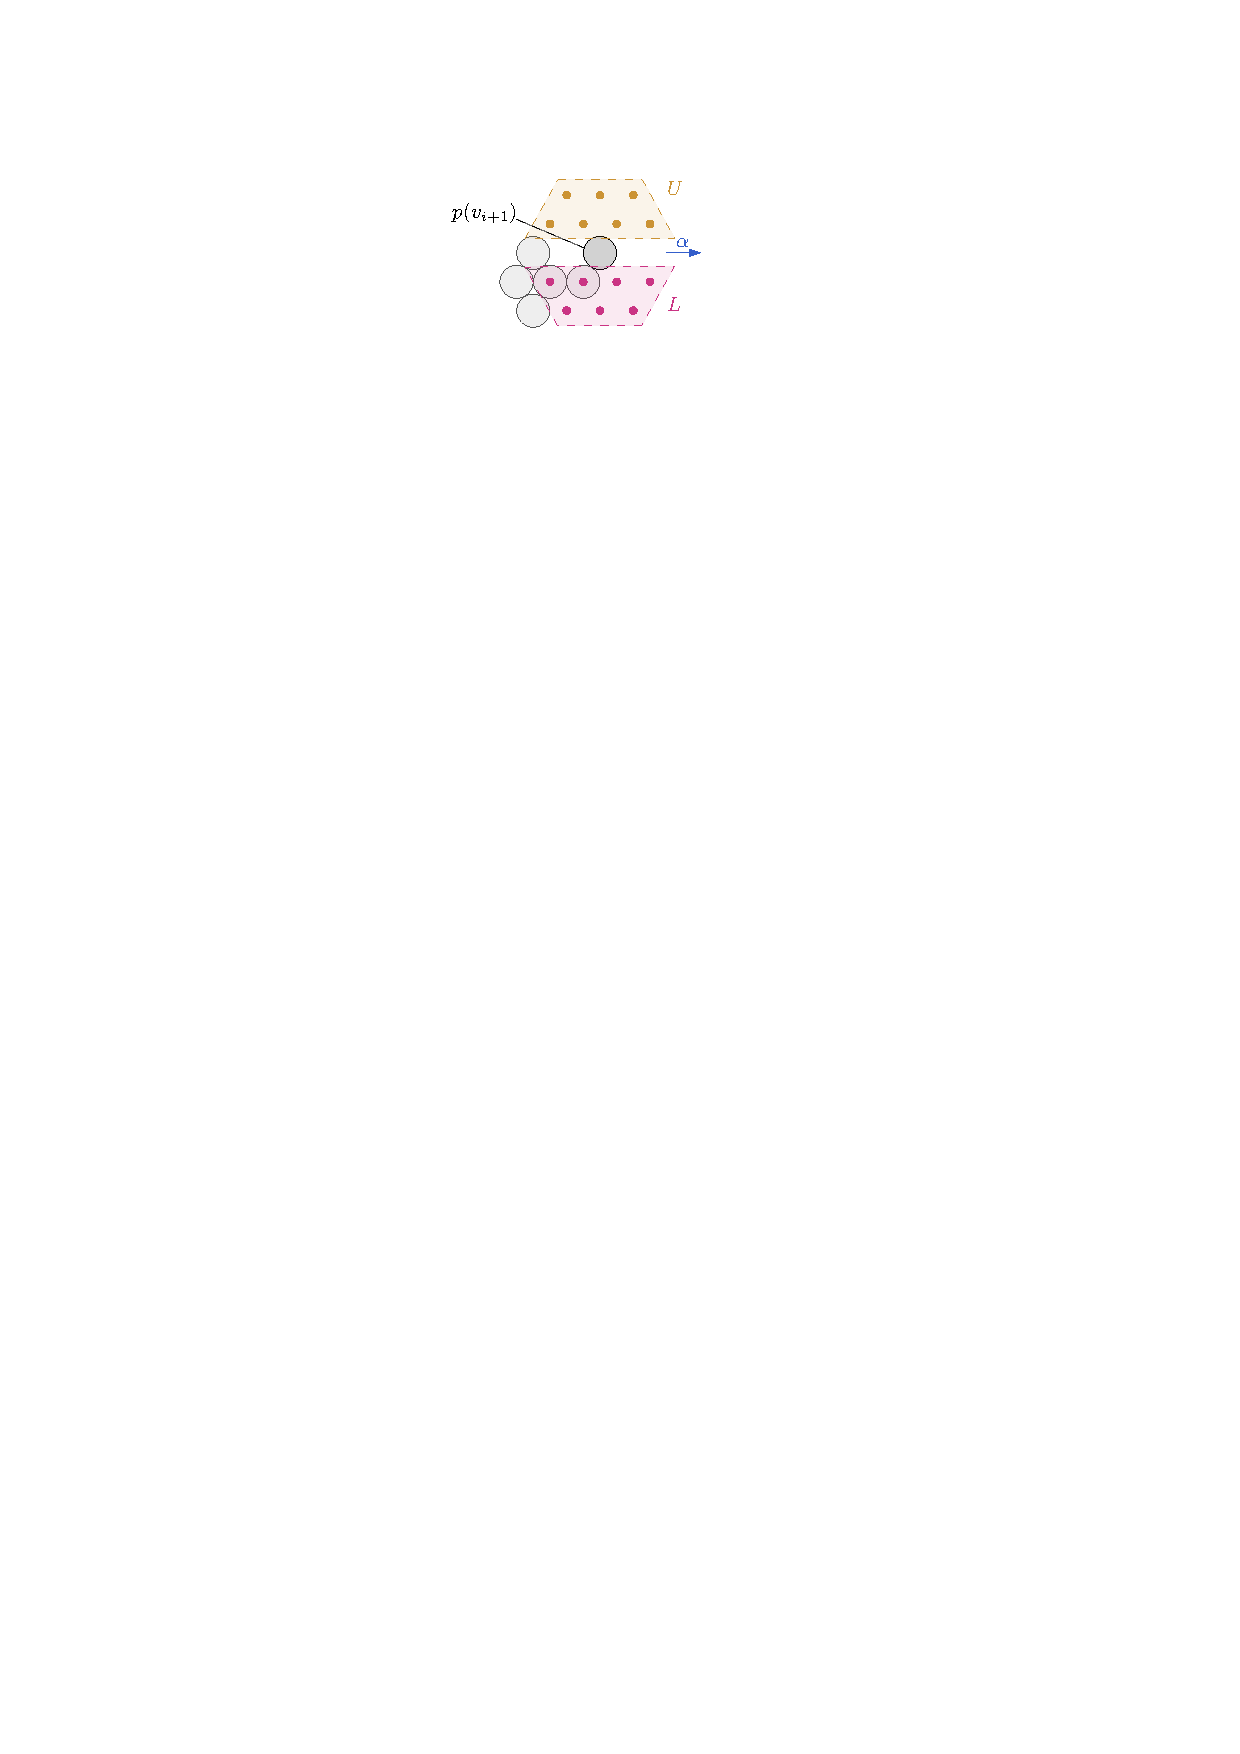
\includegraphics{ch5_affinity.pdf}
\end{figure}
\end{column}
\end{columns}

\end{frame}

\begin{frame}{Breadth-First Order}

\begin{figure}
    %\setlength{\unitlength}{0.14in} % selecting unit length
    \centering % used for centering Figure
    \scalebox{1}{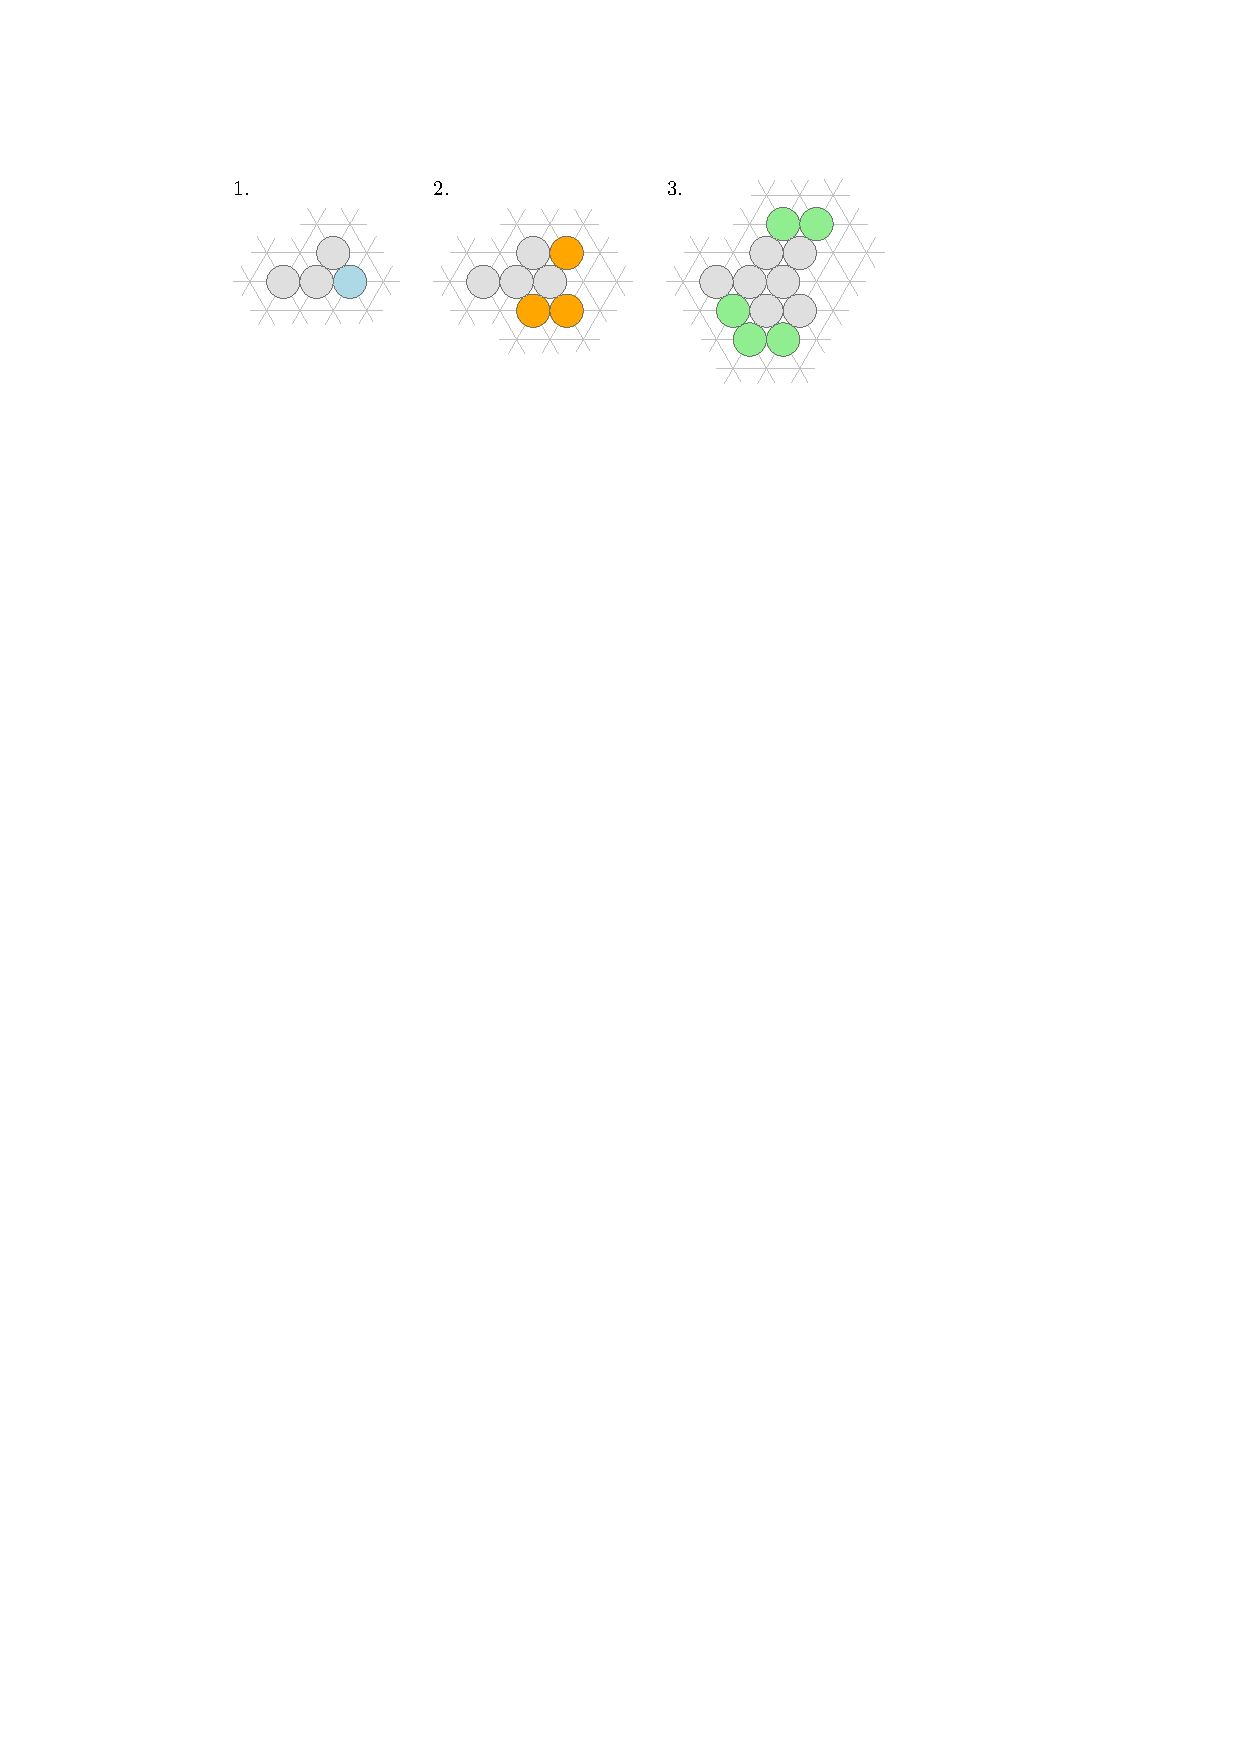
\includegraphics{slide-graphics/ch5_bfs.pdf}}
\end{figure}


\end{frame}


\section{Evaluation}

\begin{frame}{Enumerating Instances}

$$d_{1,1}d_{1,2}d_{1,3}d_{1,4}d_{1,5}\_d_{2,1}d_{2,2}d_{2,3}d_{2,4}d_{2,5}\_\ldots\_d_{n,1}d_{n,2}d_{n,3}d_{n,4}d_{n,5}$$

\begin{columns}
\begin{column}{0.01\textwidth}
\end{column}
\begin{column}{0.4\textwidth}
    \begin{itemize}
    \item Interpretation as base-6 number
    \item Count up; next digit on failure
    \item Branch ordering
    \item Orientation
    \item Dominance
    \item Heuristic-based skip
    \end{itemize}
\end{column}
\begin{column}{0.57\textwidth}
\begin{figure}
    \centering
    \scalebox{.8}{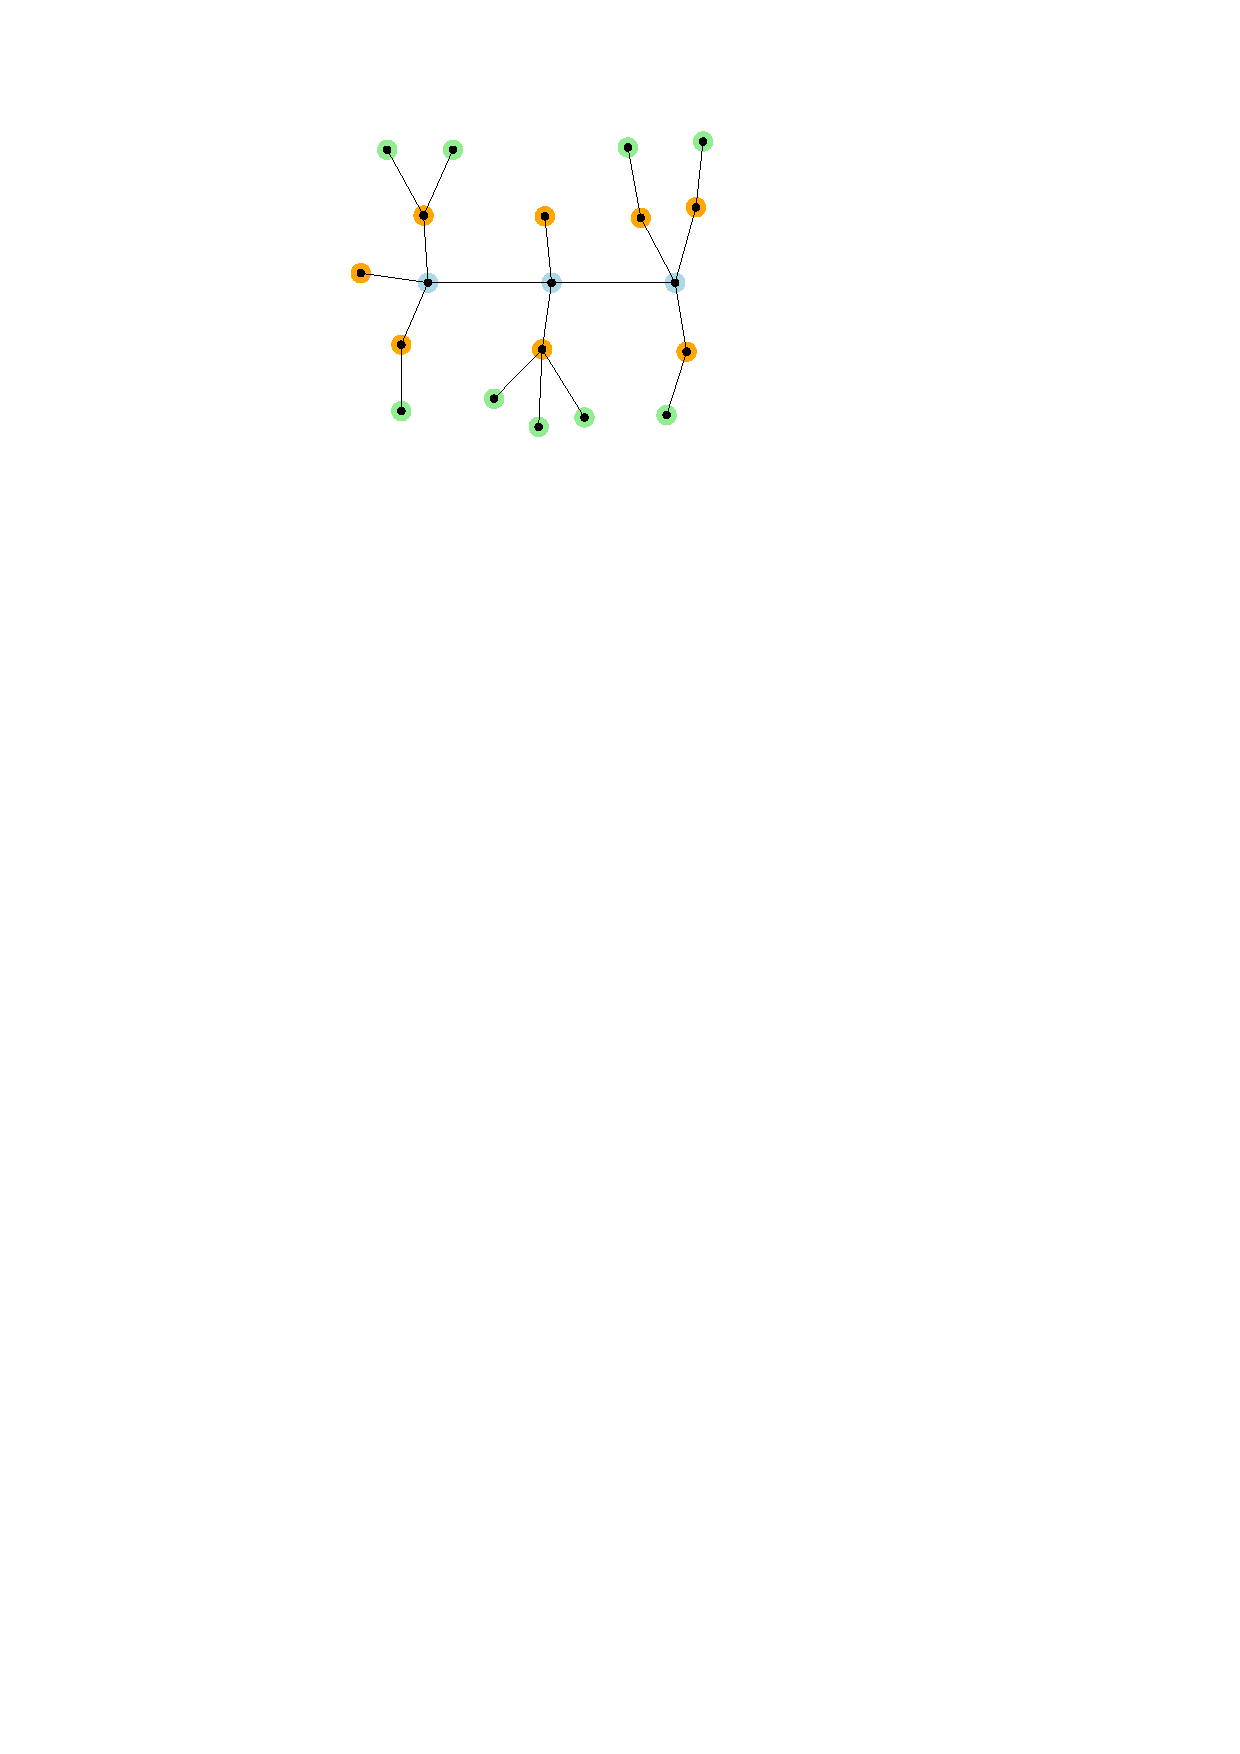
\includegraphics{ch6_degree_notation.pdf}}
    \caption*{Degree Notation: $210xx\_30xxx\_111xx$}
\end{figure}
\end{column}
\end{columns}

\end{frame}

\begin{frame}{Experiment on Lobsters up to 7 Spines}

\begin{table}
\centering
\begin{tabular}{ r|r|r }
\toprule
Spine Length & Yes-Instances & No-Instances \\
 \hline
2	 & 141	 	& 101 	\\
3	 & 1107	 	& 757 	\\
4	 & 9343	 	& 6297 	\\
5	 & 80952	& 54336  \\
6	 & 698352	& 468667  \\
7	 & 6041183	& 4053036  \\
\bottomrule
\end{tabular}
\end{table}

\end{frame}

\begin{frame}{Dynamic Program Runtime}

\begin{figure}
    \centering

    % Legend left of plots
% \begin{tabular}{@{}c@{}c@{}c@{}}
%     \noindent\parbox[c]{.11\textwidth}{\ref{legend:runtime-dp}} &
%     \begin{minipage}{0.44\textwidth}\scalebox{1}{\includestandalone[]{standalone/runtime-dp}}\end{minipage} & 
%     \begin{minipage}{0.40\textwidth}\scalebox{1}{\includestandalone[]{standalone/runtime-dpyes}}\end{minipage}
% \end{tabular}

    % Legend below plots
    \scalebox{.8}{\includestandalone[]{standalone/runtime-dp}}
    \scalebox{.8}{\includestandalone[]{standalone/runtime-dpyes}}
    \ref{legend:runtime-dp}
\end{figure}

\end{frame}

\begin{frame}{Heuristic Runtime}

\begin{figure}

    % Legend left of plots
% \begin{tabular}{@{}c@{}c@{}}
%     \begin{minipage}{\textwidth}\scalebox{.9}{\includestandalone[]{slide-graphics/runtime-dfs}}\end{minipage}&
%     \noindent\parbox[c]{.11\textwidth}{\ref{legend:runtime-heuristic}}
% \end{tabular}

    % Legend below plots
    \begin{tabular}{@{}cc@{}}
    \scalebox{.9}{\includestandalone[]{slide-graphics/runtime-dfs}}
    &
    \parbox[c]{.11\textwidth}{\vspace{-190pt}\ref{legend:runtime-heuristic}}
    \end{tabular}
\end{figure}

\end{frame}

\begin{frame}{Heuristic Runtime (Windows System)}

\begin{figure}
    \begin{tabular}{@{}cc@{}}
    \scalebox{1}{\includestandalone[]{slide-graphics/runtime-dfs-alternative}}
    &
    \parbox[c]{.11\textwidth}{\vspace{-190pt}\ref{legend:runtime-heuristic-alternative}}
    \end{tabular}
    
\end{figure}

\end{frame}

\begin{frame}{Dynamic Program vs Heuristic}

\begin{figure}
    \begin{tabular}{@{}cc@{}}
    \scalebox{1}{\includestandalone[]{slide-graphics/runtime-dp-vs-h_1}}
    &
    \parbox[c]{.11\textwidth}{\vspace{-200pt}\ref{legend:runtime-dp-vs-h}}
    \end{tabular}
\end{figure}

\end{frame}

\begin{frame}{Heuristic Accuracy}

\begin{figure}
    %\setlength{\unitlength}{0.14in} % selecting unit length
    \centering % used for centering Figure
    \scalebox{1}{\includestandalone[]{slide-graphics/accuracy_1}}
\end{figure}

\end{frame}

\begin{frame}{Conclusion}

\begin{itemize}
\item Two algorithms with custom improvements
\item Heuristic: up to $250\times$ speedup, $70\%$ solved for 7 spines
\item Open Question: $60^{\circ}$-Monotonicity?
\end{itemize}

\makebox[0pt][l]{%
  \raisebox{-80pt}[0pt][0pt]{\hspace*{130pt}%
    \scalebox{.1}{\includesvg{slide-graphics/onesided_bent20.txt.svg}}}}%

  % \centering\Huge
  % Thank You

\end{frame}

\begin{frame}[allowframebreaks]
        \frametitle{References}
        
\AtNextBibliography{\footnotesize}
        \printbibliography
\end{frame}

\end{document}
